\documentclass[aspectratio=169,10pt]{beamer}
\usepackage{amsmath,amssymb}
\usepackage{booktabs}
\usepackage{graphicx}
\usepackage{listings}
\usepackage{xcolor}
\usepackage{hyperref}

% Theme
\usetheme{Madrid}
\usecolortheme{default}

% Title info
\title{FlashAttention: GPU-Efficient Attention}
\subtitle{CS290W LLM07 Lecture}
\author{LU Yuzhou}
\date{}

% Code listing style
\definecolor{codebg}{RGB}{245,245,245}
\lstset{
    backgroundcolor=\color{codebg},
    basicstyle=\ttfamily\scriptsize,
    frame=single,
    breaklines=true,
    keywordstyle=\color{blue},
    commentstyle=\color{gray},
    stringstyle=\color{red},
    showstringspaces=false,
    upquote=true,
    literate={__}{{\texttt{\_}\texttt{\_}}}2
             {->}{{$\to$}}2
             {=>}{{$\Rightarrow$}}2,
}

\begin{document}

% Title slide
\frame{\titlepage}

% Slide 1: Overview
\begin{frame}{The Problem: Attention is Memory-Bound}
    \begin{itemize}
        \item Standard self-attention has $O(N^2)$ HBM memory access
        \item HBM (High-Bandwidth Memory) = slow off-chip DRAM
        \item For long sequences, memory bandwidth is the bottleneck, not FLOPs
    \end{itemize}

    \vspace{0.3cm}
    \textbf{FlashAttention Solution:} Leverage GPU memory hierarchy to minimize HBM access

    \vspace{0.3cm}
    \begin{block}{Key Insight}
        On-chip SRAM (shared memory) is $\sim 10\times$ faster than HBM. Keep intermediate results on-chip!
    \end{block}

    \vspace{0.3cm}
    \begin{center}
        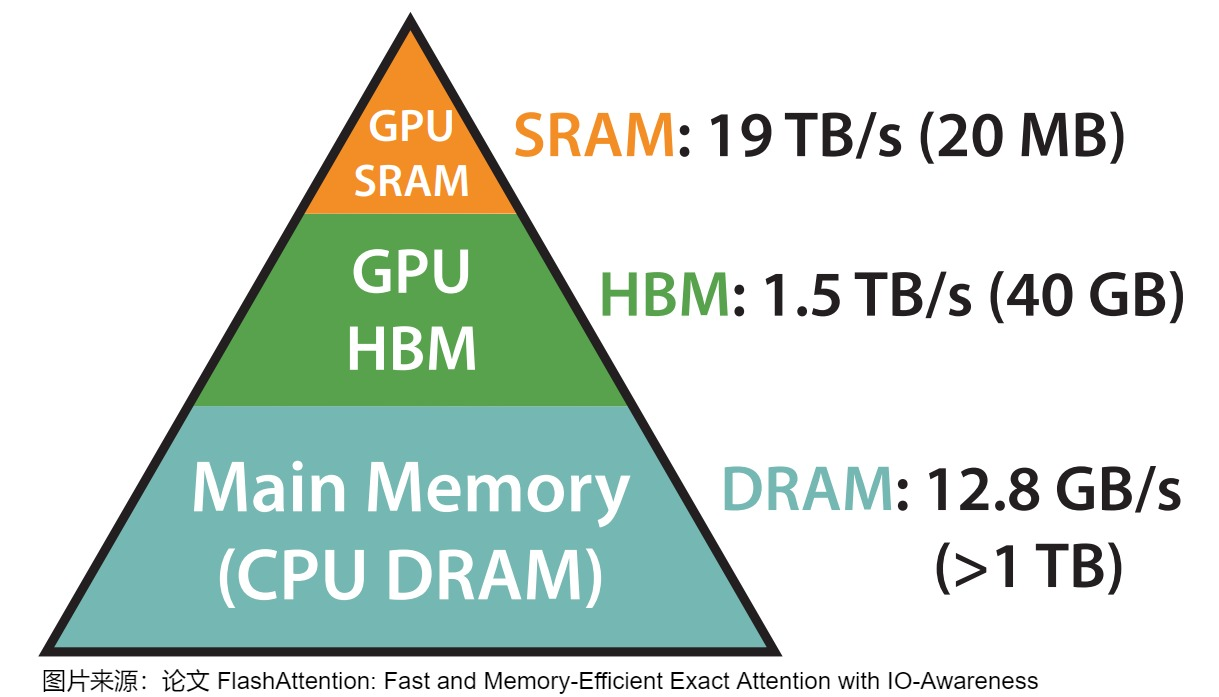
\includegraphics[width=0.3\textwidth]{img/07-01-gpu-memory-hierarchy.jpg}
    \end{center}
\end{frame}

% Slide 2: GPU Memory Hierarchy
\begin{frame}{GPU Memory Hierarchy}
    \begin{table}
        \centering
        \small
        \begin{tabular}{lrrr}
            \toprule
            \textbf{Level} & \textbf{Size (A100)} & \textbf{Bandwidth} & \textbf{Latency} \\
            \midrule
            Registers & ~256 KB / SM & --- & ~1 cycle \\
            Shared Memory (SRAM) & 164 KB / SM & ~19 TB/s & ~30 cycles \\
            L2 Cache & 40 MB & ~5 TB/s & ~200 cycles \\
            HBM (Global) & 80 GB & 2.0 TB/s & ~400+ cycles \\
            \bottomrule
        \end{tabular}
    \end{table}

    \vspace{1cm}
    \begin{itemize}
        \item Shared memory bandwidth: \textbf{19 TB/s} vs HBM: \textbf{2 TB/s}
        \item Goal: Minimize HBM round-trips by keeping intermediates in SRAM
    \end{itemize}


\end{frame}

% Slide 2b: Measuring Actual Bandwidth
\begin{frame}[fragile]{Measuring Actual Memory Bandwidth}
    \textbf{Lab Exercise:} Measure HBM/GDDR bandwidth on your machine using tensor copy:

    \vspace{0.3cm}
    \begin{lstlisting}[language=Python]
def measure_memory_bandwidth(device, size_mb=256):
    num_elements = int(size_mb * 1e6 / 4)  # float32
    src = torch.randn(num_elements, device=device)

    # Benchmark tensor clone (HBM read + write)
    t0 = time.perf_counter()
    for _ in range(repeats):
        _ = src.clone()
    elapsed = (time.perf_counter() - t0) / repeats

    bandwidth = (num_elements * 4 / elapsed) / 1e9  # GB/s
    return bandwidth
    \end{lstlisting}

    \vspace{0.3cm}
    \begin{block}{Example Result (RX 7900 XTX)}
        HBM Bandwidth: \textbf{391 GB/s} (measured) \\
        SRAM Bandwidth: \textbf{19,000 GB/s} (typical) \\
        → SRAM is $\sim 49\times$ faster!
    \end{block}
\end{frame}

% Slide 3: Standard Attention IO Analysis
\begin{frame}{Standard Attention IO Analysis: Why $O(N^2)$ HBM Access?}
    For sequence length $N$ and head dimension $d$:

    \begin{enumerate}
        \item Read $Q, K$ from HBM → Compute $S = QK^T$ → \textbf{Write $S$ to HBM}
        \item Read $S$ → Compute $P = \text{softmax}(S)$ → \textbf{Write $P$ to HBM}
        \item Read $P, V$ → Compute $O = PV$ → Write $O$ to HBM
    \end{enumerate}

    \vspace{0.1cm}
    \begin{block}{Total HBM Access}
        $O(Nd + N^2)$ — dominated by the $N \times N$ matrices $S$ and $P$
    \end{block}

    \vspace{0.1cm}
    Example: $N=4096$, FP16 → Score matrix = \textbf{33.6 MB per head}


    \begin{center}
        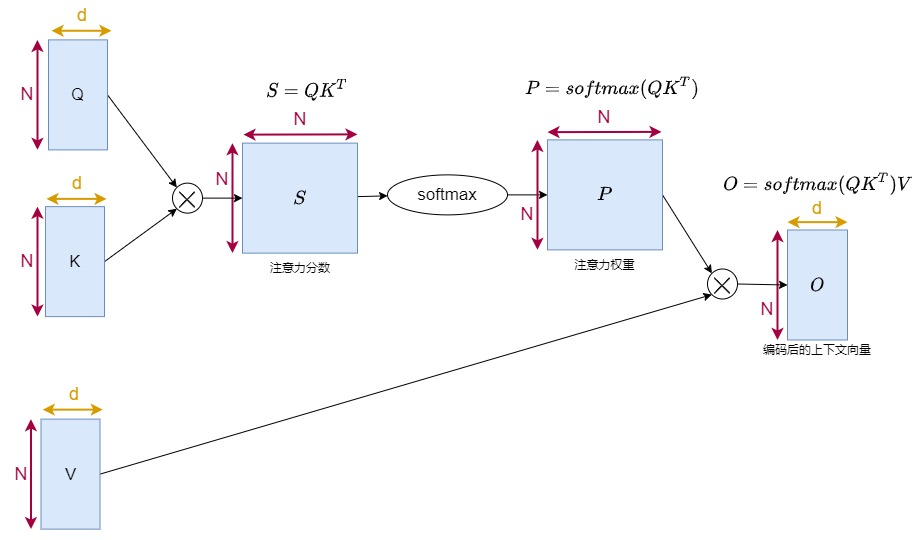
\includegraphics[width=0.4\textwidth]{img/07-06-operator-fusion.jpg}
    \end{center}
\end{frame}

% Slide 4: Tiling for Matrix Multiplication
\begin{frame}{Optmization 1# Tiling: Partitioning for SRAM}
    \textbf{Tiling} partitions matrices into blocks that fit in shared memory.

    \vspace{0.3cm}
    \begin{itemize}
        \item Each tile is loaded \textbf{once} from HBM
        \item Reused for multiple computations in SRAM
        \item Example: 32×32 matmul with 16×16 tiles
        \item Global memory reads: $65{,}536 \to 4{,}096$ (\textbf{16× reduction})
    \end{itemize}


\end{frame}

% Slide 4b: HIP Kernel for Tiled MatMul
\begin{frame}[fragile]{HIP Kernel: Tiled Matrix Multiplication}
    Real GPU implementation using HIP:

    \vspace{0.3cm}
    \begin{lstlisting}[language=C++]
__global__ void tiledMatMul(float* A, float* B, float* C) {
    __shared__ float As[TILE][TILE];
    __shared__ float Bs[TILE][TILE];

    int tx = threadIdx.x, ty = threadIdx.y;
    int row = blockIdx.y * TILE + ty;
    int col = blockIdx.x * TILE + tx;
    float sum = 0.0f;

    for (int t = 0; t < numTiles; t++) {
        // Load tiles from HBM to SRAM
        As[ty][tx] = A[row * K + t*TILE + tx];
        Bs[ty][tx] = B[(t*TILE + ty) * N + col];
        __syncthreads();  // Wait for all threads

        // Compute in SRAM (fast!)
        for (int k = 0; k < TILE; k++)
            sum += As[ty][k] * Bs[k][tx];
        __syncthreads();
    }
    C[row * N + col] = sum;
}
    \end{lstlisting}


\end{frame}

% Slide 5: What is Softmax?
\begin{frame}{Normal Softmax: Two-Pass Algorithm}
    \textbf{Softmax} converts real numbers to a probability distribution:

    \vspace{0.1cm}
    $$\text{softmax}(x)_i = \frac{e^{x_i}}{\sum_{j=1}^{N} e^{x_j}}$$

    \vspace{0.1cm}
    \textbf{Numerical Stability:} Subtract max to prevent overflow:
    $$\text{softmax}(x)_i = \frac{e^{x_i - m}}{\sum_{j=1}^{N} e^{x_j - m}}, \quad m = \max_j x_j$$

    \vspace{0.2cm}
    \begin{block}{Two-Pass Algorithm}
        \textbf{Pass 1 (REDUCE):} Find $m = \max(x)$, compute $s = \sum e^{x_j - m}$ \\
        \textbf{Pass 2 (MAP):} For each $i$: $p_i = e^{x_i - m} / s$\
    \end{block}
\end{frame}

% Slide 5b: Softmax Resource Analysis
\begin{frame}{Softmax Resource Analysis}
    \begin{table}
        \centering
        \small
        \begin{tabular}{llll}
            \toprule
            \textbf{Step} & \textbf{Operation} & \textbf{Type} & \textbf{Resource} \\
            \midrule
            Pass 1, Step 1 & $m = \max(x)$ & REDUCE & Memory-bound \\
            Pass 1, Step 2 & $s = \sum e^{x_j - m}$ & REDUCE & Memory-bound \\
            Pass 2, Step 3 & $p_i = e^{x_i - m} / s$ & MAP & Compute-bound \\
            \bottomrule
        \end{tabular}
    \end{table}

    \vspace{0.5cm}
    \textbf{Key Observations:}
    \begin{itemize}
        \item \textbf{REDUCE operations} are memory-bound: must read entire input from HBM
        \item \textbf{MAP operation} is compute-bound: exponential + division per element
        \item Total HBM traffic: $O(N)$ per row → \textbf{$O(N^2)$ for full attention matrix}
    \end{itemize}

    \vspace{0.5cm}
    \begin{block}{Problem}
        Standard softmax must \textbf{materialize full $N \times N$ matrix} in HBM \\
        For $N=4096$: 33.6 MB per head — too large for SRAM!
    \end{block}
\end{frame}

% Slide 6: Online Softmax Algorithm
\begin{frame}{Online Softmax: Single-Pass Solution}
    \begin{block}{Challenge for Attention}
        Row-wise softmax depends on the \textbf{entire row}. Cannot compute softmax per-tile until all tiles are seen.
    \end{block}


    \textbf{Online softmax} maintains running statistics $(m, d)$ updated incrementally:

    \vspace{0.3cm}
    \begin{table}
        \centering
        \small
        \begin{tabular}{lll}
            \toprule
            \textbf{Property} & \textbf{Standard} & \textbf{Online} \\
            \midrule
            Passes & 2 (must see all data) & 1 (streaming) \\
            State & Full input stored & Only $(m, d)$ — 2 values! \\
            Use Case & Small vectors & Large matrices (attention) \\
            \bottomrule
        \end{tabular}
    \end{table}

    \vspace{0.5cm}
    \textbf{Update Formulas:}
    \begin{align*}
        m_{\text{new}} &= \max(m_{\text{old}}, m_{\text{block}}) \\
        d_{\text{new}} &= d_{\text{old}} \cdot e^{m_{\text{old}} - m_{\text{new}}} + \sum_{j \in \text{block}} e^{x_j - m_{\text{new}}}
    \end{align*}

\end{frame}

% Slide 7: FlashAttention V1 Algorithm
\begin{frame}{FlashAttention V1: Core Algorithm}
    Process $Q, K, V$ in \textbf{tiles}:

    \vspace{0.3cm}
    \begin{enumerate}
        \item Divide $K, V$ into blocks of $B_c$ rows; $Q$ into blocks of $B_r$ rows
        \item For each Q-block, iterate over K/V-blocks:
        \begin{itemize}
            \item Load Q-tile, K-tile, V-tile into SRAM
            \item Compute local $S_{\text{tile}} = Q_{\text{tile}} K_{\text{tile}}^T$
            \item Update running softmax (online softmax)
            \item Accumulate output: $O \mathrel{+}= \text{softmax\_tile} \times V_{\text{tile}}$
        \end{itemize}
        \item Final rescaling after all blocks
    \end{enumerate}

    \vspace{0.5cm}
    \begin{block}{HBM Access Complexity}
        $O(N^2 d^2 / M)$ where $M$ = SRAM size — much less than $O(Nd + N^2)$
    \end{block}

    \vspace{0.3cm}

\end{frame}
\begin{frame} {FlashAttention V1: Diagram}
        \begin{center}
        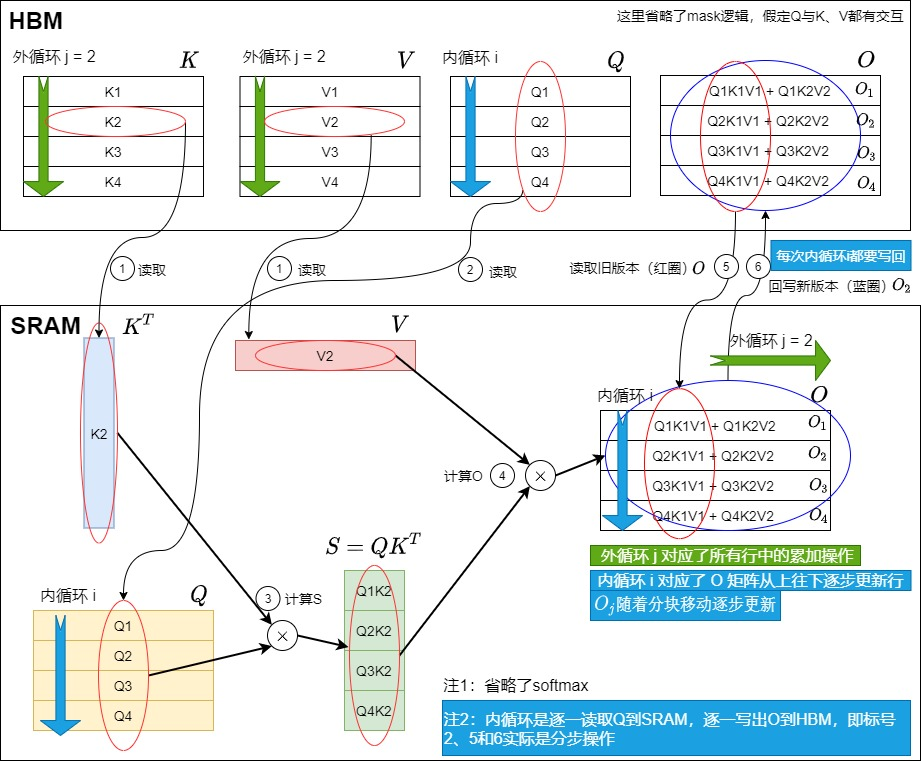
\includegraphics[width=0.55\textwidth]{img/07-17-v1-forward-pass.jpg}
    \end{center}
\end{frame}

% Slide 8: FlashAttention V1 vs V2 Comparison
\begin{frame}[fragile]{FlashAttention V1 vs V2: Why V2 is Faster}
    \textbf{V1 Pseudocode (K/V-outer):}
    \vspace{0.2cm}
    \begin{lstlisting}
for j in K/V_blocks:              # Outer: K/V
    for i in Q_blocks:            # Inner: Q
        S_tile = Q[i] @ K[j].T
        m_new = max(m[i], m_tile)
        O[i] *= exp(m[i] - m_new) # RESCALE EVERY ITER!
        O[i] += exp(S_tile) @ V[j]
    \end{lstlisting}

    \vspace{0.3cm}
    \textbf{V2 Pseudocode (Q-outer):}
    \vspace{0.2cm}
    \begin{lstlisting}
for i in Q_blocks:                # Outer: Q
    for j in K/V_blocks:          # Inner: K/V
        S_tile = Q[i] @ K[j].T
        m_new = max(m[i], m_tile)
        O[i] += exp(S_tile) @ V[j] # NO RESCALE!
    O[i] /= l[i]                  # FINAL RESCALE ONLY
    \end{lstlisting}

    \vspace{0.3cm}

\end{frame}

\begin{frame}{FlashAttention V1 vs V2: Why V2 is Faster? (Continued)}
        \begin{block}{V2 Advantages}
        \textbf{Deferred rescaling:} $O(N)$ writes vs $O(N^2)$ \\
        \textbf{Better locality:} Each SM owns Q-block, processes all K/V \\
        \textbf{No inter-warp sync:} Q-split instead of K-split
    \end{block}

    \vspace{0.3cm}
    \begin{center}
        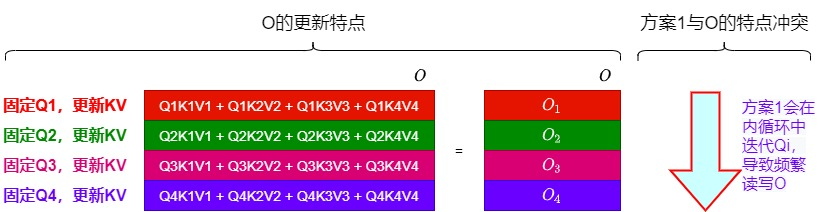
\includegraphics[width=0.7\textwidth]{img/07-18-io-complexity.jpg}
    \end{center}
\end{frame}

% Slide 9: IO Complexity Comparison
\begin{frame}{IO Complexity Comparison}
    \begin{table}
        \centering
        \small
        \begin{tabular}{lrr}
            \toprule
            \textbf{Method} & \textbf{HBM Reads/Writes} & \textbf{Peak HBM} \\
            \midrule
            Standard Attention & $O(Nd + N^2)$ & $O(N^2)$ \\
            FlashAttention V1 & $O(N^2 d^2 / M)$ & $O(N)$ \\
            FlashAttention V2 & Same, fewer ops & $O(N)$ \\
            \bottomrule
        \end{tabular}
    \end{table}

    \vspace{0.5cm}
    Where:
    \begin{itemize}
        \item $M$ = SRAM size per SM (~100-200 KB)
        \item $N$ = sequence length
        \item $d$ = head dimension (typically 64-128)
    \end{itemize}

    \vspace{0.3cm}
    \begin{block}{Key Takeaway}
        For typical settings ($d=64$--$128$, $M \gg d^2$), FlashAttention eliminates \textbf{almost all $N^2$-sized HBM traffic}
    \end{block}


\end{frame}

% Slide 10: Memory Savings Example
\begin{frame}{Memory Savings: Real Numbers}
    Intermediate memory per head (FP16, $d=128$):

    \vspace{0.3cm}
    \begin{table}
        \centering
        \small
        \begin{tabular}{rrrr}
            \toprule
            \textbf{$N$} & \textbf{Standard} & \textbf{Flash} & \textbf{Savings} \\
            \midrule
            512 & 0.52 MB & 0.0008 MB & 655× \\
            1024 & 2.10 MB & 0.0016 MB & 1311× \\
            2048 & 8.39 MB & 0.0031 MB & 2687× \\
            4096 & 33.55 MB & 0.0063 MB & 5338× \\
            8192 & 134.22 MB & 0.0125 MB & 10701× \\
            \bottomrule
        \end{tabular}
    \end{table}

    \vspace{0.5cm}
    \begin{block}{Why This Matters}
        Standard attention runs out of memory for long sequences. \\
        FlashAttention enables \textbf{context lengths of 64K+} on consumer GPUs.
    \end{block}
\end{frame}

% Slide 11: PyTorch Integration
\begin{frame}[fragile]{Using FlashAttention in PyTorch}
    PyTorch $\geq$ 2.0 provides automatic FlashAttention via SDPA:

    \vspace{0.3cm}
    \begin{lstlisting}[language=Python]
import torch.nn.functional as F

# SDPA automatically uses FlashAttention when available
output = F.scaled_dot_product_attention(Q, K, V)
    \end{lstlisting}

    \vspace{0.5cm}
    \begin{itemize}
        \item \texttt{scaled\_dot\_product\_attention} (SDPA) selects backend:
        \begin{itemize}
            \item FlashAttention (ROCm/CUDA)
            \item Memory-Efficient Attention
            \item Math fallback
        \end{itemize}
        \item No code changes needed!
    \end{itemize}

    \vspace{0.3cm}
    \begin{block}{Dedicated Library}
        \texttt{pip install flash-attn} → \texttt{flash\_attn\_func(Q, K, V)}
    \end{block}
\end{frame}

% Slide 12: Benchmark Results
\begin{frame}{Benchmark: Standard vs Flash Attention}
    Typical speedups on modern GPUs (A100, H100, RX 7900 XTX):

    \vspace{0.3cm}
    \begin{table}
        \centering
        \small
        \begin{tabular}{rrrr}
            \toprule
            \textbf{$N$} & \textbf{Standard} & \textbf{SDPA (Flash)} & \textbf{Speedup} \\
            \midrule
            256 & 0.15 ms & 0.12 ms & 1.25× \\
            512 & 0.45 ms & 0.28 ms & 1.61× \\
            1024 & 1.52 ms & 0.78 ms & 1.95× \\
            2048 & 5.89 ms & 2.45 ms & 2.40× \\
            4096 & 23.45 ms & 7.82 ms & 3.00× \\
            \bottomrule
        \end{tabular}
    \end{table}

    \vspace{0.5cm}
    \begin{itemize}
        \item Speedup increases with sequence length
        \item Memory savings: \textbf{2--5×} lower peak HBM usage
    \end{itemize}


\end{frame}

% Slide 13: Summary
\begin{frame}{Summary: Key Takeaways}
    \begin{enumerate}
        \item \textbf{GPU Memory Hierarchy}: SRAM is 10× faster than HBM
        \item \textbf{Tiling}: Partition computation to fit in SRAM
        \item \textbf{Softmax Analysis}: REDUCE is memory-bound, MAP is compute-bound
        \item \textbf{Online Softmax}: Single-pass with running stats $(m, d)$
        \item \textbf{FlashAttention V1}: $O(N^2 d^2 / M)$ HBM vs $O(N^2)$ standard
        \item \textbf{FlashAttention V2}: Deferred rescaling, Q-outer loop, better warp usage
    \end{enumerate}

    \vspace{0.5cm}
    \begin{block}{Bottom Line}
        FlashAttention is not about reducing FLOPs — it's about \textbf{reducing memory traffic}. \\
        This makes it \textbf{2--4× faster} and enables \textbf{longer context lengths}.
    \end{block}
\end{frame}

% Slide 14: Further Exploration
\begin{frame}{Experiment Further}
    \begin{itemize}
        \item Install \texttt{flash-attn} package: \texttt{pip install flash-attn}
        \item Compare FP16 vs BF16 performance
        \item Benchmark causal masks (autoregressive) vs bidirectional
        \item Profile with \texttt{torch.profiler} to see SRAM/HBM usage
        \item Read the papers:
        \begin{itemize}
            \item FlashAttention V1: \href{https://arxiv.org/abs/2205.14135}{arXiv:2205.14135}
            \item FlashAttention V2: \href{https://arxiv.org/abs/2307.08691}{arXiv:2307.08691}
        \end{itemize}
    \end{itemize}

    \vspace{0.5cm}
    \begin{block}{Lab Notebook}
        See \texttt{LLM07-FlashAttention.ipynb} for hands-on exercises: \\
        - Measure memory bandwidth \\
        - Implement tiled matmul (Python + HIP) \\
        - Implement online softmax \\
        - Simulate FlashAttention V2 \\
        - Benchmark standard vs SDPA
    \end{block}

\end{frame}


